\section{Processor Optimizations}
\label{sec:processor_opt}

Our processor optimizations are based on arithmetic operations, such as addition and multiplication, which are performance critical in training computations, and have predetermined results when one of the input operands is a zero. We refer to machine instructions that perform such arithmetic operations as ``zero-optimizable'' instructions. Exploiting zero-optimizable instructions to improve training peformance is promising because, as shown in our profiling studies (Figure~\ref{fig:cifar-10_word_sparsity}), a significant portion of the inputs to training computations are zeroes. 

\begin{figure*}
\centering
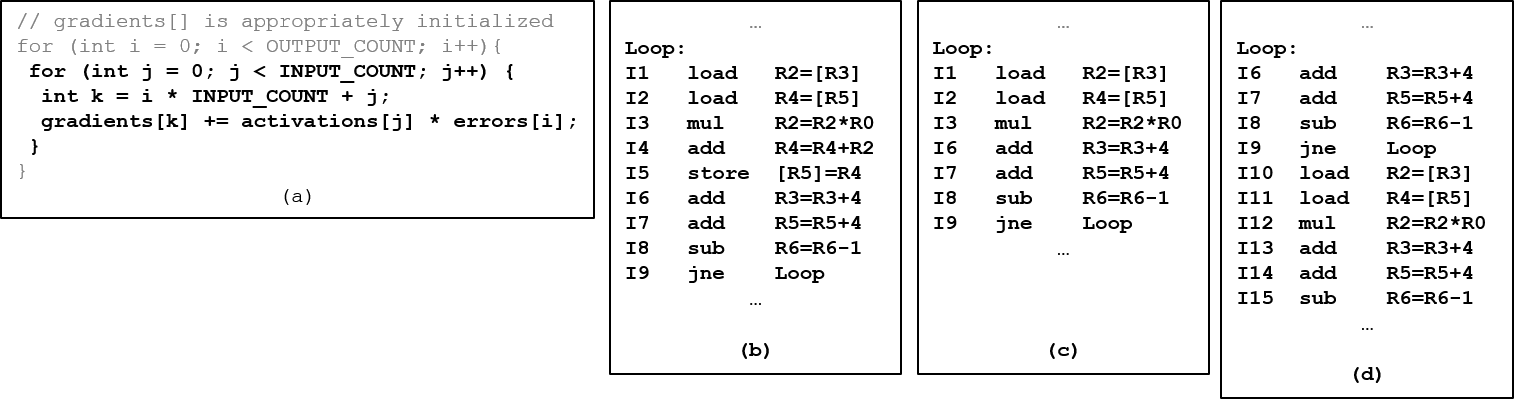
\includegraphics[width=1.9\columnwidth]{Figures/gradient_code_opt.png}
\caption{(a) Source code for computing gradients, (b) machine code of inner loop, (c) optimized code after basic instruction quashing, and (d) optimized code after advanced instruction quashing.}
\label{fig:gradient_code_opt}
\end{figure*}

\subsection{Sample Training Computation.}

We will use the training code snippets shown in Figure~\ref{fig:gradient_code_opt} to describe our optimizations.  Figure~\ref{fig:gradient_code_opt}(a) illustrates a simplifed version of the performance critical code for computing weight gradients of a layer during back-propagation. Gradients are computed as an inner product of the activation and error vectors. A promising optimization for this code is to skip multiply and addition operations in the inner loop if \emph{activations[j]} or \emph{errors[i]} is zero. Also, when \emph{errors[i]} is zero then the inner loop can be skipped. 

Although this optimization could be implemented in software, that approach has a couple of practical limitations.   First, it requires software changes which might not be possible for existing binaries.   Second, the overheads of the required software checks for zeroes could be significant and outweigh the optimization benefits.  For example,  the performance impact of checking \emph{errors[i]} and \emph{activations[j]} are quite different.  Checking \emph{errors[i]} is likely to be beneficial because it is done outside the inner loop and helps to skip large amount of computation. In contrast, checking \emph{activations[j]} will likely degrade performance because it occurs inside the inner loop and can provide small amount of computation savings. Our hardware optimizations  avoid these limitations.  We compare the performance benefits of software and hardware  approaches in our evaluation. 

\subsection{Zero-Optimizable Instructions.}

Zero-optimizable instructions present a number of opportunities to increase ILP and reduce resource pressure of training computations on modern out-of-order processors.  These opportunities arise because of the predetermined results of zero-optimizable instructions when computing with zero input operands.  In this paper, our focus are zero-optimizable instructions that perform additions or multiplications.  Thus, for concreteness we consider how these instructions could be affected by a zero input when there are two input and one output operands.  

 A zero input operand converts an addition instruction into a copy operation of the other input operand into the destination location. Also, if the other input operand is also the destination operand then the copy operation is redundant.  For multiplications, a zero input operand results in a zero value of the destination operand regardless of the value of the other input operand.  Thus, zero input operands can make some data dependencies and pipeline stages redundant for zero-optimizable and dependent instructions.  Consequently, zero-optimizable and dependent instructions can be issued or commited earlier than normal or skipped completely, as discussed below. 


\subsection{Opportunities}

We illustrate our optimizations using the machine code sequences in  Figures~\ref{fig:gradient_code_opt}(b), ~\ref{fig:gradient_code_opt}(c), and ~\ref{fig:gradient_code_opt}(d), which correspond to the original and optimized versions of the inner loop.  Although there are five zero-optimizable instructions in the loop (I$3$, I$4$, I$6$, I$7$, and I$8$), the optimizations discussed invole only I$3$ and I$4$. We assume that R$0$, which corresponds to \emph{errors[i]}, is zero. 


\subsubsection{Early Instruction Issue/Commit.}  First, a zero-optimizable instruction can be issued once the zero operand is available if it makes other operands redundant.  For example, I$3$ can be issued early becaue it is a multiplication and the zero value of R$0$ makes R$2$ redundant.  Second, a zero-optimizable instruction could be committed early if the zero input determines its results and side effects. This is also the case for I$3$. Early issue and commit of zero-optimizable instructions can reduce pressure on processor resources and wait times of data dependent instructions, such as I$4$, since the dependencies are satisfied sooner. 

\subsubsection{Instruction Squashing.} A zero-optimizable instruction can be squashed in the instruction queue if a zero input operand makes it an identity function and thus redundant. For this reason, I$4$ can be squashed since it is an addition and R$2$ is zero. Squashing an instruction can make the  instructions that it depends on (producers) and those that depend on it (consumers) redundant, leading to more instruction squashing.  For example, I$5$ becomes redundant (a silent store) and can be squashed, if I$5$ is squashed. Figure~\ref{fig:gradient_code_opt}(c) shows the impact of squashing I$4$ and I$5$.  We further observe that  I$1$, I$2$, and I$3$ are now redundant in all but the last loop iteration, since their results (R$2$ and R$4$) are not used.  We can squash these three instructions in all but the last iteration as shown in Figure~\ref{fig:gradient_code_opt}(d). Compared to the orignal machine code sequence, the optimized code sequence will run much faster because of the squashed instructions, especially loads which often have high latency.  Thus, by exploiting zero-optimizable instructions we can improve the performance of the inner loop of the gradient computation code. 

\subsection{Mechanisms}

We propose extensions to a modern OOO pipeline for dynamic optimization of zero-optimizable instructions and the loops containing them.  Our optimizer system comprises of lightweight extensions in the front-end and heavyweight extensions in the back-end of the pipeline.  The split into lightweight and heavyweight components helps to avoid critical path delays in the front-end, while extracting maximum performance improvements.  The front-end extensions enable early instruction issue/commit, while the back-end extensions enable instruction squashing in loops.  Figure~\ref{fig:opt_pipeline} presents an overview of augmenting a standard OOO six-stage pipeline with our optimization system.

\begin{figure}
\centering
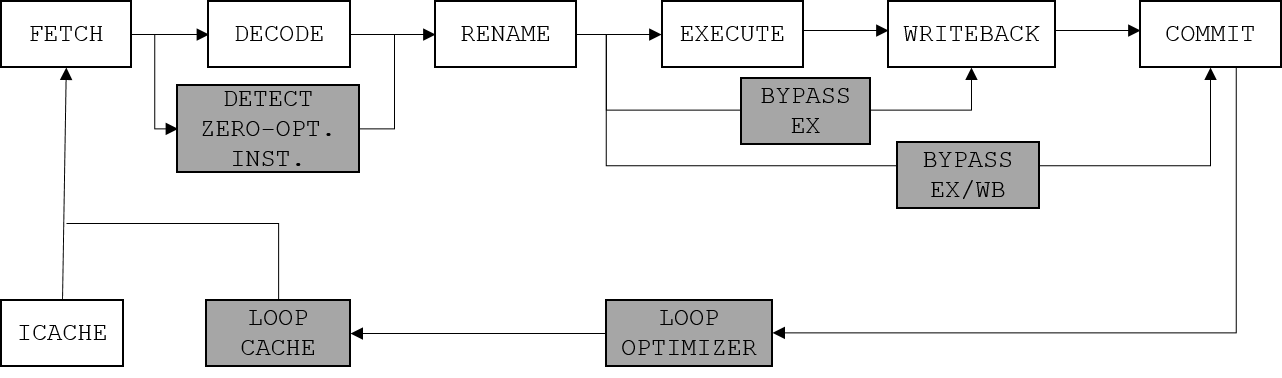
\includegraphics[height=1in]{Figures/pipeline.png}
\caption{Overview of processor extensions.}
\label{fig:opt_pipeline}
\end{figure}

\subsubsection{Front-End Extensions.}
The objectives of the front-end extensions are the following: (i) detect zero-optimizable instructions in the instruction stream and (ii) bypass pipeline stages.  These steps can be done in parallel with existing pipeline stages, as discussed below.  

\paragraph{Detect Zero-optimizable Instructions.}
This is done in the decode stage by matching the instruction opcode against a predefined set of opcodes. Since the opcode set is small, i.e., addition and multiplication opcodes, the matching can be done in parallel to avoid extra delays.  The zero-optimizable instructions detected here are marked for easy identification in later pipeline stages. 

\paragraph{Bypass Pipeline Stages.}
We exploit zero operand values to bypass the execute and writeback stages whenever possible.  This is done while a zero-optimizable instruction is in the instruction queue waiting for data dependencies.  We extend the mechanism for detecting operand availability to also check whether or not the value is zero.  For a multiplication instruction or a redundant addition instruction (i.e., destination operand is same as other source operand), we break outstanding data dependencies of the instruction making the instruction ready to issue.  We extend the issue logic to allowing issuing instructions directly to stages later than the execute stage.  This allows us to issue multiplication instructions to the writeback stage to zero the destination operand (and broadcast availability), and issue redundant additions to the commit stage.   

%Our approach performs the following operations in the pipeline front-end: (i) identify zero-optimizable instructions, (ii) detect when zero-optimizable input operand is a zero, (iii) modify producer and consumer data dependencies, and (iv) squash instructions.  These steps can be done in parallel with existing pipeline front-end stages, as we discuss below. 

%\subsubsection{Identify Zero-Optimizable Instructions.} We can detect zero-optimizable instructions during instruction decoding by matching the opcode against a predefined set of opcodes. Since only a small set of arithmetic instructions qualify as zero-optimizable, the storage requirements of the opcode set is modest, and opcode matching can be done in parallel to avoid extra delays. Zero-optimizable instructions that are identified in the decode stage are marked for easy identification in later pipeline stages. 

%\subsubsection{Detect Zero Operands.} We can detect zero input operands while a zero-optimizable instruction is waiting in the instruction queue for data dependencies.  Current mechanisms for signaling operand availability can be extended to also indicate whether or not the value is zero. 
 
 %\subsubsection{Modify Data Dependencies.}  We can extend current mechanisms for tracking data dependencies among instructions to clear dependencies of zero-optimizable instructions that become redundant due to a zero input operand becoming available. Futhermore, dependencies from instructions that consume the results of a zero-optimizable instruction should be cleared when a zero input makes the instruction an identity function, and thus redundant.  
 
 \subsubsection{Back-End Extensions.}
 Our backend extensions consists of two components: (i) a mechanism for detecting and optimizing loops based on zero-optimizable instructions, and (ii) an optimized loop code cache.  The goal is to eliminate instructions that are made redundant by zero inputs to zero-optimizable instructions in the loop.  Thus, the optimized loop code is smaller than the original loop 
 
 \paragraph{Loop Optimizer.} This mechanism scans the stream of committed instructions to detect loops that can be optimized based on zero-optimizable 
 
 \paragraph{Optimized Loop Code Cache.}
 
 
